%\begin{center}
%\begin{tikzpicture}
%  \coordinate (O) at (0,0);

%  % ball background color
%  \shade[ball color = white, opacity = 0.2] (0,0) circle [radius = 2cm];

%  % cone
%  \begin{scope}
%    \def\rx{0.2}% horizontal radius of the ellipse
%    \def\ry{0.05}% vertical radius of the ellipse
%    \def\z{3}% distance from center of ellipse to origin
    
%    \path [name path = ellipse]    (0,\z) ellipse ({\rx} and {\ry});
%    \path [name path = horizontal] (-\rx,\z-\ry*\ry/\z)
%                                -- (\rx,\z-\ry*\ry/\z);
%    \path [name intersections = {of = ellipse and horizontal}];

%    % radius to base of cone in ball
%    \draw[fill = gray!50, densely dashed] (intersection-1) -- (0,0)
%      -- (intersection-2) -- cycle;
%    % base of cone in ball
%    \draw[fill = gray!30, densely dashed] (0,\z) ellipse ({\rx} and {\ry});
%  \end{scope}

%  % label of cone
%  \draw (0.25,0.4) -- (0.9,0.1) node at (1.05,0.0) {$q$};

%  % ball
%  \draw (O) circle [radius=2cm];
%  % label of ball center point
%  \filldraw (O) circle (1pt) node[below] {$P$};

%  % radius
%  \draw[densely dashed] (O) to [edge label = $r$] (-1.33,1.33);
%  \draw[densely dashed] (O) -- (1.33,1.33);

%  % label of cut of ball surface
%  \draw (-1.2,2.2) -- (-0.53,1.83) node at (-1.37,2.37) {$A$};
%\end{tikzpicture}\end{center}

\begin{center}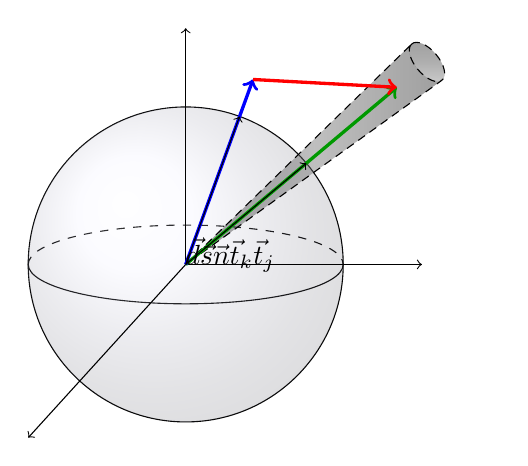
\begin{tikzpicture}
	% circle
    \draw (-2,0) arc (180:360:2cm and 0.5cm);
    \draw[dashed] (-2,0) arc (180:0:2cm and 0.5cm);
    %\draw (0,1) arc (90:270:0.5cm and 1cm);
    %\draw[dashed] (0,1) arc (90:-90:0.5cm and 1cm);
    \draw (0,0) circle (2cm);
    \shade[ball color=blue!10!white,opacity=0.20] (0,0) circle (2cm);
    	%cone
    \fill[rotate=-50, top color=gray!50!black,bottom color=gray!10,middle color=gray,shading=axis,opacity=0.25] (0,4) circle (0.3cm and 0.15cm);
    \fill[rotate=-50,left color=gray!50!black,right color=gray!50!black,middle color=gray!50,shading=axis,opacity=0.25] (-0.3,4) -- (0,0) -- (0.3,4) arc (360:180:0.3cm and 0.15cm);
    \draw[rotate=-50,densely dashed](-0.3,4) arc (180:360:0.3cm and 0.15cm) -- (0,0) -- cycle;
    \draw[rotate=-50,densely dashed] (-0.3,4) arc (180:0:0.3cm and 0.15cm);
    
    	%coordinate system
    \coordinate (O) at (0,0);
    \coordinate (x) at (-2,-2.2);
    \coordinate (z) at (0,3);
    \coordinate (y) at (3,0);
    \draw [->] (O)--(z);
    \draw [->] (O)--(y);
    \draw [->] (O)--(x);
    
% convert using this site: http://keisan.casio.com/exec/system/1223522781  
    	% t_j vectors
    \coordinate (d) at (2.681,2.2498); % (0,3.5)
    \coordinate (s) at (0.855,2.349); % (0, 2.5) rotated 20 degrees
    \draw [very thick,->,color=green!60!black] (O)--(d);
    \draw [very thick, ->,color=blue] (O)--(s);
    \draw [very thick, ->,color=red] (s)--(d);
    \coordinate (tk) at (1.532,1.2856); % (0,2)
    \coordinate (tj) at (0.684,1.8794); % (0, 2) rotated -20 degrees
    \draw [->] (O)--(tk);
    \draw [->] (O)--(tj);
    
    \tkzLabelSegment[right=10.5pt,color=green!60!black,pos=0.68](O,d){$\vec{d}$};
    \tkzLabelSegment[left,color=blue,pos=0.92](O,s){$\vec{s}$};
    \tkzLabelSegment[above,color=red](s,d){$\vec{n}$};
    \tkzLabelSegment[right=7pt](O,tk){$\vec{t}_k$};
    \tkzLabelSegment[left,pos=0.7](O,tj){$\vec{t}_j$};
    
    \node [right] at (3.2,2.7){$\Delta\Omega$};
    
\end{tikzpicture}
\end{center}
